
% this file is called up by thesis.tex
% content in this file will be fed into the main document

%: ----------------------- introduction file header -----------------------
%************************************************
\chapter{Introduction}\label{ch:introduction}
%************************************************

% the code below specifies where the figures are stored
\ifpdf
    \graphicspath{{1_introduction/figures/PNG/}{1_introduction/figures/PDF/}{1_introduction/figures/}}
\else
    \graphicspath{{1_introduction/figures/EPS/}{1_introduction/figures/}}
\fi

% ----------------------------------------------------------------------
%: ----------------------- introduction content ----------------------- 
% ----------------------------------------------------------------------



%: ----------------------- HELP: latex document organisation
% the commands below help you to subdivide and organise your thesis
%    \chapter{}       = level 1, top level
%    \section{}       = level 2
%    \subsection{}    = level 3
%    \subsubsection{} = level 4
% note that everything after the percentage sign is hidden from output

\section{Motivation}

The need to use robotic systems in order to overcome human beings' limitations
has been a topic of an ever increasing interest in the last decades. Manipulator
arms, for instance, were introduced in the industry to optimize production lines
by systematically executing tasks with a bounded margin of error and high
repeatability during long working hours. Recently, such an interest in robots
has veered towards autonomous vehicles that conduct missions in complex and
undiscovered environments, such as deep oceans, volcanoes and even other
planets. Consequently, various sectors of the scientific community started to
research this area, especially focused on developing robotic vehicles that are
capable of conducting tasks where data is gathered autonomously in different
environmental media, such as air, soil and water~\cite{Dunbabin2012}.

Marine scientists were probably the first ones capitalizing on the use of
robotic vehicles in exploring unknown environments. Oceanographers, for
instance, started using \acp{UUV} to study deep marine environments and the
seafloor~\cite{Whitcomb2000}. Nowadays, \acp{UUV} are separated into two
categories according to the level of human intervention required for their
operation. A first group includes the so-called \acp{ROV} which, despite being
unmanned, have to be tethered to a support surface vessel from which they are
powered and controlled by a human operator. Although \acp{ROV} are commonly
associated with their use in inspecting and maintaining offshore oil and gas
platforms~\cite{Khan2002}, they have also contributed to different scientific
applications such as environmental monitoring~\cite{Lam2006} and marine
archeology~\cite{Forney2011}. Figure~\ref{fig:rov} shows the widely-known VICTOR
6000 \ac{ROV} in a typical deployment maneuver from the mother ship, where the
umbilical cable used to operate the vehicle can be clearly observed.

\begin{figure}[htbp]
\centering
	\subfloat[]{
		\label{fig:victor6000-rov}
        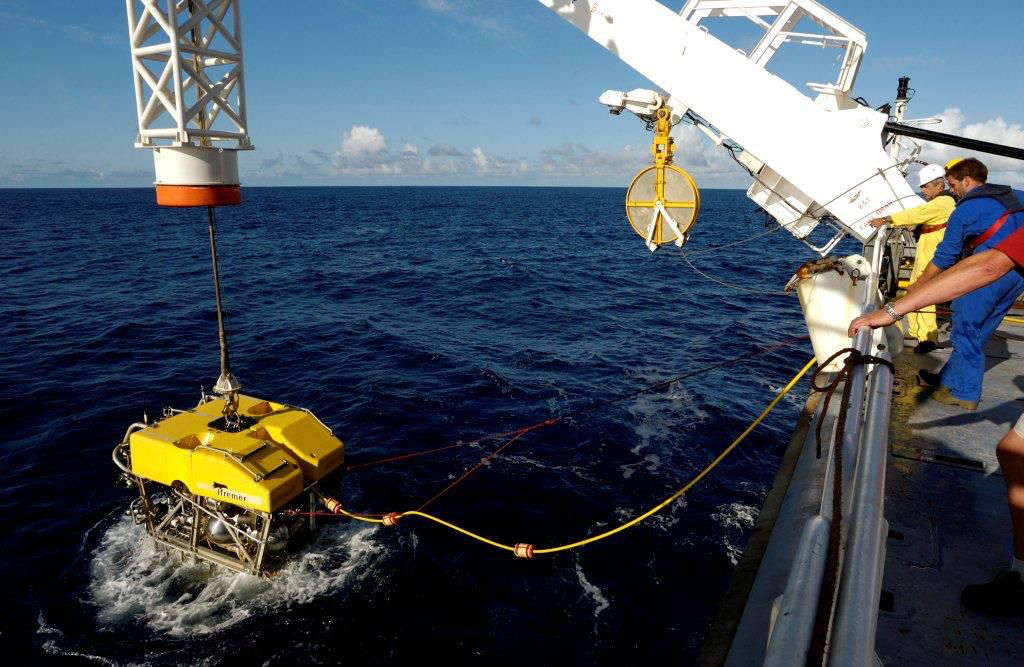
\includegraphics[width=.45\linewidth]{Victor6000-ROV}} \quad
	\subfloat[]{
		\label{fig:Victor6000-ROV-Ship}
		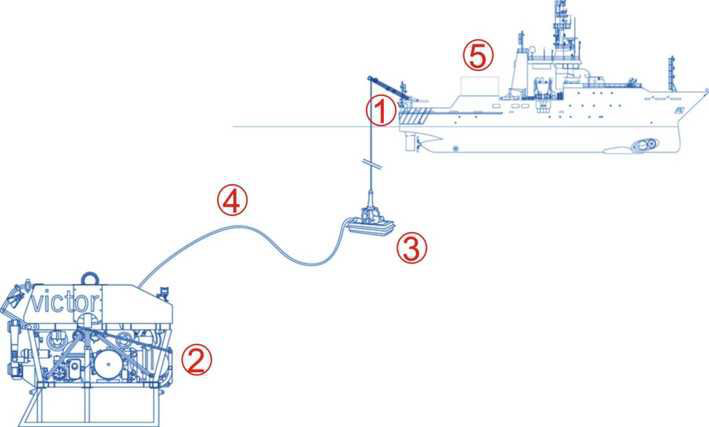
\includegraphics[width=.45\linewidth]{Victor6000-ROV-Ship}}
\caption[VICTOR 6000: a remotely operated vehicle (ROV) and its surface vessel.]
{\subref{fig:victor6000-rov} The VICTOR 6000 ROV.
\subref{fig:Victor6000-ROV-Ship} The ROV-vessel system: 1) a direct-winding
winch, 2) the ROV, 3) the hard ballast, 4) the tether
cable, and 5) the power/hydraulic units and control room. Image
credit: Ifremer.
%\url{http://flotte.ifremer.fr/fleet/Presentation-of-the-fleet/Underwater-systems/VICTOR-6000}
}
\label{fig:rov}
\end{figure}

The second group gathers the \acp{AUV}, or \acp{UUV} that do not require being
controlled by a human operator. This characteristic eliminates the need of
continuously being in contact with a surface mother ship, thus permitting to
overcome some major drawbacks of the former group, such as their high operative
cost and limited working area. In most of the \ac{AUV} applications, the vehicle
follows a sequence of pre-calculated waypoints and uses its onboard sensors to
gather oceanographic information of biological nature~\cite{Grasmueck2006},
chemical composition~\cite{WeiLi2006}, and even archaeological
data~\cite{Bingham2010}. Often, they are also equipped with multibeam and
imaging sonars that collect data that is used to build bathymetric maps
(\ie elevation maps of the seabed). These underwater surveys are normally
conducted in a previously explored area so that the vehicle navigates at a
constant and safe altitude from the seafloor.

Furthermore, \acp{AUV} can also be divided into two main subcategories:
buoyancy-driven and propeller-driven. The former category corresponds to the
underwater gliders, or \acp{AUV} that are capable of modifying its buoyancy in
order to generate sinusoidal-like vertical motion that, together with their
wings, also permit horizontal (forward and lateral) motion. The trajectories
followed by these vehicles also include periodic ascents to the surface to
obtain GPS fixes, thus improving its navigation estimation (see
Fig.~\ref{fig:GliderAUV}). This propulsion technique results in a
low-consumption but also less maneuverable approach. This is commonly used in
long-term studies over open sea areas, in which a single mission can last from
days to weeks.

\begin{figure}[htbp]
	\centering
	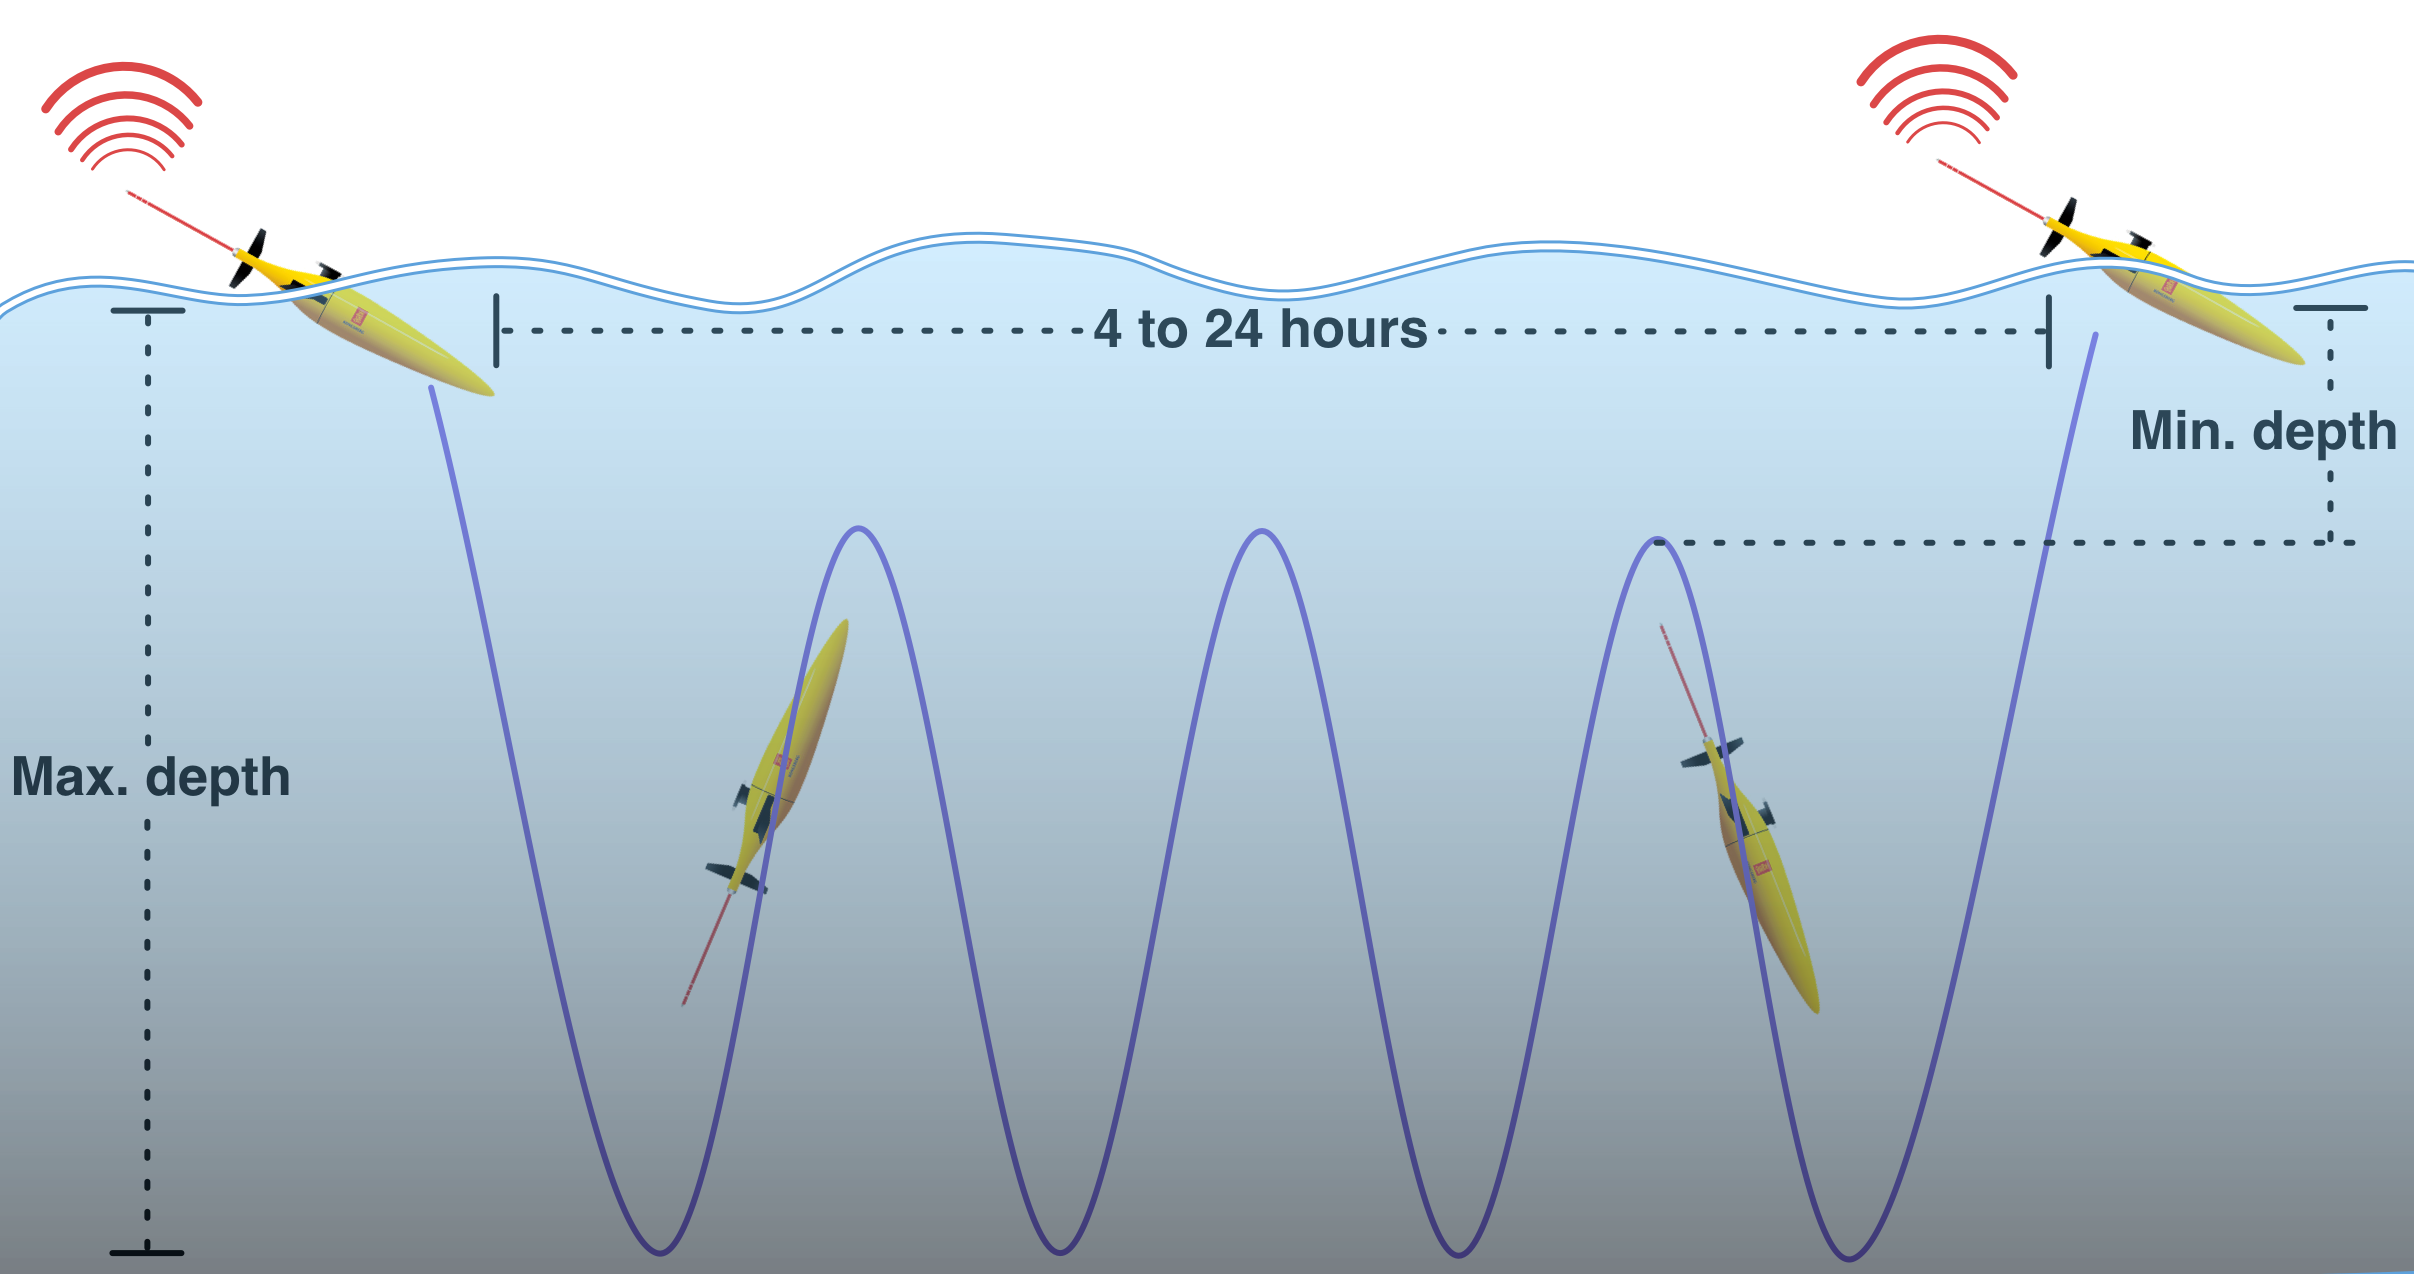
\includegraphics[width=.8\linewidth]{SeagliderAUV} \quad
\caption[Underwater glider and its sinusoidal-like vertical motion.]
{Underwater glider, or AUV with the capability of modifying its buoyancy to
generate sinusoidal-like vertical motion. The vehicle dives for several hours to
gather data, and surfaces periodically to obtain GPS fixes thus improving its
own navigation estimation.}
\label{fig:GliderAUV}
\end{figure}

The propeller-driven \acp{AUV}, on the other hand, correspond to those that use
propellers or thrusters to generate \ac{3D} motions. The work presented
throughout this thesis is dedicated to this latter kind of vehicles.
Furthermore, it has been mainly validated with the Sparus~II, a torpedo-shaped
\ac{AUV} (see Fig.~\ref{fig:Sparus2}).

\begin{figure}[htbp]
	\centering
	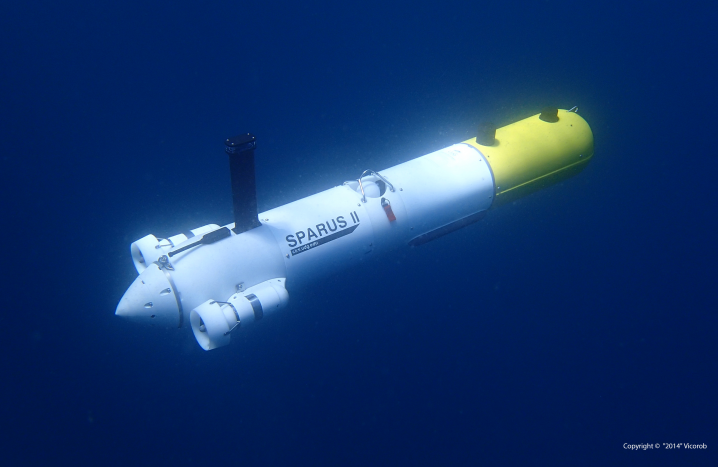
\includegraphics[width=.6\linewidth]{Sparus2} \quad
\caption[Sparus~II: a torpedo-shaped and propeller-driven autonomous underwater
vehicle (AUV).]
{Sparus~II AUV, a torpedo-shaped and propeller-driven underwater vehicle, which
is equipped with two back thrusters for horizontal motion, and one independent
thruster for vertical motion.}
\label{fig:Sparus2}
\end{figure}

% \begin{figure}[bth]
%         \myfloatalign
%         \subfloat[Asia personas duo.]
%         {\includegraphics[width=.45\linewidth]{gfx/example_1}} \quad
%         \subfloat[Pan ma signo.]
%         {\label{fig:example-b}%
%          \includegraphics[width=.45\linewidth]{gfx/example_2}} \\
%         \subfloat[Methodicamente o uno.]
%         {\includegraphics[width=.45\linewidth]{gfx/example_3}} \quad
%         \subfloat[Titulo debitas.]
%         {\includegraphics[width=.45\linewidth]{gfx/example_4}}
%         \caption[Tu duo titulo debitas latente]{Tu duo titulo debitas
%         latente. \ac{DRY}}\label{fig:example}
% \end{figure}

\section{Problem Statement}

Recent \ac{AUV} applications include imaging and inspecting different kinds of
structures such as in-water ship hulls~\cite{Hover2012,Hurtos2015} and natural
structures on the sea floor~\cite{Galceran2014b}. These applications share a
common characteristic: they require \textit{a priori} information of the area or
structure to be inspected. Therefore it is needed to either navigate at a safe
and conservative altitude~\cite{Grasmueck2006,Bingham2010} or to pre-calculate a
survey path that may be corrected or reshaped
online~\cite{Hover2012,Galceran2014b}. However, there are similar or even
potentially new applications, such as exploring confined natural environments
(\eg underwater caves)~\cite{Mallios2015}, where such information might not be
available. In these scenarios, the \ac{AUV} must operate in unexplored
(unknown), cluttered and dynamic environments, and therefore are more exposed to
collisions.

Although the aforementioned \ac{AUV} applications share some common requirements
with aerial and terrestrial robots (\eg localization, mapping, vision, etc.),
navigating autonomously while conducting such type of tasks in an underwater
environment presents different challenges. These are caused by factors specific
to this environment, such as the presence of external disturbances (currents),
low-range visibility and limited navigation accuracy. Dealing with such
constraints requires a path planner with online computation capabilities, which
contribute in overcoming the lack of surroundings information and the global
position inaccuracy, especially when navigating in close proximity to nearby
obstacles.

\subsection{Navigating in Unexplored Environments with AUVs}

Even with the most recent technological advances, conducting both teleoperated
and autonomous missions in underwater environments still represents a challenge
with different scientific aspects to be solved. One important restriction faced
by \acp{UUV} is that they operate in GPS-denied environments, which limits their
capability to accurately calculate their position with respect to an inertial
reference frame. In order to cope with this, \ac{DR} techniques are used to
estimate the relative position with respect to an initial position, which is
normally defined from GPS fixes obtained when the vehicle is at surface. This
approach suffices in many survey \ac{AUV} applications. However, its limitations
rely on highly precise odometry and low-level or negligible disturbances. When
these conditions are not met, it can rapidly lead to errors in distance
estimation, which make this approach an unsafe alternative when navigating and
exploring surroundings in close proximity to nearby obstacles, even when the
environment is known and a map is available.

Another alternative is the of use of an \ac{USBL}, which is a method of
underwater acoustic positioning. An \ac{USBL} system is composed of a
transceiver mounted on a surface vessel and a transponder mounted on the
\ac{AUV}. This system permits calculating the range (distance) and the angle of
the subsea vehicle with respect to the surface vehicle. Furthermore, given that
the transceiver is at surface (\ie it can get GPS fixes), it is possible to
calculate a more accurate absolute position of the \ac{AUV}. The major drawback
of this alternative is the mobility constraint imposed by the transceiver,
similar to what occurs with a \ac{ROV} and its mother ship. This also prevents
its use in confined natural environments such as an underwater caves complex,
which results in a critical limitation for the new applications intended for
\acp{AUV}.

Therefore, when planning collision-free \ac{AUV} paths, the difficulty to
pre-explore and build a map of the area or structure of interest is an
additional challenge to be considered together with the navigation inaccuracy.
In order to tackle these problems, this thesis proposes a framework that endows
an \ac{AUV} with the capability to map an undiscovered environment, while
planning collision-free paths to navigate throughout it. Furthermore, although
the framework considers specific characteristics of the motion planning problem
for \acp{AUV}, the proposed approach may also be applied for other types of
autonomous vehicles.

\subsection{Path/Motion Planning Problem for AUVs}

\subsubsection{Overview of the Basic Robot Path/Motion Planning}

In general, path/motion planning methods can be divided into two categories
according to their application: coverage planning and start-to-goal planning.
The former category, commonly referred to as \ac{CPP}, gathers those methods
that seek to determine a collision-free path that a robot must follow in order to
pass over all points of an area or volume of interest. A detailed review of
available techniques that address this problem can be found
in~\cite{Galceran2013a}.

The second category, \ie start-to-goal motion planning, consists in finding
valid (collision-free) paths from a start configuration to a goal configuration
in the \ac{C-Space}, which is the space of all the possible robot
configurations~\cite{Lozano-Perez1983}. There are different computational
algorithms that attempt to solve this task. Some of them find an analytic
solution, but their applicability is limited to simple problems. Another group
of algorithms, such as Dijkstra's~\cite{Dijkstra1959}, A*~\cite{Hart1968} and
D*~\cite{Stentz1994}, search throughout discretization of the \ac{C-Space}.
However, in problems involving high-dimensional \acp{C-Space}, these exhaustive
search methods suffer from scalability issues.

One alternative in dealing with this is to use the so-called sampling-based
methods. These latter ones construct a partial representation by taking samples
at random from the \ac{C-Space} and checking them for
collisions~\cite{Choset2005,LaValle2006}, instead of fully describing the
\ac{C-Space}. In contrast with exhaustive search methods, these are not complete
(\ie they can not report whether a solution exists), but often find a
solution for complex problems where other algorithms fail.

There are additional characteristics or capabilities that should be considered
when solving path/motion planning tasks for \acp{AUV}. Some of which will be
mentioned in the following sections.

\subsubsection{Planning under Geometric and Differential (Motion) Constraints}
\label{sec:PlannUnderConst}

When calculating a valid path, the planner must deal with different types of
constraints, some of which may be related only to the \ac{C-Space}, while others
may also include the vehicle motion capabilities. Depending on which constraints
are considered, the planning problem was categorized in one of two possible
groups: geometric path planning and motion planning ~\cite{Choset2005}. The
former group assumes that the robotic system can move instantaneously in any
direction (\ie system kinematics and dynamics are negligible), thus reducing the
problem to geometric constraints that are solved by checking for collisions over
the \ac{C-Space}.

However, the motion constraints associated with the vehicle are often
significant, and therefore the robot is not capable of following a simple
geometric path. This means that, when calculating collision-free paths, it is
necessary to use a vehicle motion model that includes differential constraints,
also called kinodynamic constraints. Such a group of planning problems is
commonly called motion planning or \textit{kinodynamic motion planning} (this
latter term was introduced by Donald \etal in 1993~\cite{Donald1993}). An
example of such planning problems is the one related to a non-holonomic
torpedo-shaped \ac{AUV}, as the ones used in this thesis (see
Figure~\ref{fig:Sparus2}).

As recently the terms path planning and motion planning are used
interchangeably~\cite{Sucan2011},~\cite{LaValle2006}, throughout this thesis, we
refer to the either problem as path/motion planning

\subsubsection{3D Path/Motion Planning}

In some \ac{AUV} applications the vehicle either navigates at constant depth or
attempts to keep reference values of altitude. In those cases, and specially in
areas with no or little relief, it is possible to simplify the motion model to
one that assumes the vertical position variation as constant or negligible.
Nonetheless, when such conditions are not met, it is required to use more
complete motion equations, which in the simplest case implies adding an
additional state variable for the vertical motion, or in more complex scenarios
may require to use a \ac{6D} state space, \ie one that incorporates the position
and the orientation of the vehicle in a \ac{3D} workspace, where each state or
configuration is $q = [x,y,z, \phi, \theta, \psi]$.
 
\subsubsection{Online Path/Motion Planning}

Another important aspect to be considered when planning motions for \acp{AUV},
especially when navigating in unexplored environments, is the necessity of
calculating the paths (motions) online. To deal with such computation
constraints, the planner must be capable of providing a solution at \textit{any
time} and of correcting (reshaping) it according to the updated environment
information gathered along the mission execution. This characteristic implies
that although it is possible that the solution provided at \textit{any time} may
not be the most optimal one, any available time left will be spent on improving
the existing solution path. This means that the next delivered solution is
better than the previous one or at least equally good. Finally, it is also
important to correctly balance the computation load to coexist with other
functional modules of the \ac{AUV} such as navigation, control, etc.

\section{Objectives of the Thesis}

Once the motivation and the most relevant aspects of the problem addressed in
this thesis have been established, the main objective of this work can be stated
as follows:

\bigskip

\noindent \textit{To endow an \acf{AUV} with the capability to incrementally map
an unexplored environment, while planning online collision-free paths; such paths
should be \acf{3D}, safe, and feasible (doable) according to the vehicle's
motion constraints. This will contribute a further step towards better and more
reliable \acp{AUV} for the new and potential applications.}

\bigskip

This objective can be separated into the following specific
objectives:

\bigskip

\noindent\textbf{Review of the Path/Motion Planning Literature:} To conduct a
review of the most relevant path/motion planning methods, which have been used
for different robotic systems including terrestrial, aerial, and, especially,
marine vehicles. This will allow identifying the most appropriate approaches for
meeting the aforementioned constraints for the intended applications.

\bigskip

\noindent\textbf{Planning Feasible Motions for AUVs:} To propose a motion
planning method that takes into account the \ac{AUV}'s motion constraints for
both 2D and 3D movements. This will permit generating more feasible motions
according to the \ac{AUV}'s capabilities. Furthermore, such motions will be more
likely to be followed by the vehicle, thus minimizing unexpected maneuvers.

\bigskip

\noindent\textbf{Online Mapping and Path/Motion Planning for AUVs:} To propose a
framework that allows an \ac{AUV} to safely navigate through initially
unexplored environments. This implies that the vehicle must be capable of
incrementally mapping the surroundings while, simultaneously and online,
planning safe and feasible paths.

\bigskip

\noindent\textbf{Simulation and In-water Validation:} To extensively test and
validate the proposed approach in different simulated and real-world scenarios.

\section{Thesis Outline and Contributions}

This manuscript is organized in a way that presents the incremental and
progressive development of this thesis. In order to contextualize and better
understand the real impact of such developments,
Chapter~\ref{ch:state_of_the_art} firstly makes a review of the most relevant
methods, techniques, and applications that compose the state of the art, not
only in what has to do with path/motion planning, but also in relation with the
approaches currently applied with \acp{AUV}. Then, based on the new and
potential applications intended for \acp{AUV} that were mentioned above, and
considering their requirements, the main contributions of this thesis are
gathered and distributed throughout this document as follows:

\begin{inparaenum}[1)]

\item The incorporation of motion constraints into the \ac{AUV} path planner,
which acts as a mechanism to avoid generating unfeasible paths, thus reducing
the number of unexpected maneuvers. This includes those constraints required for
constant depth missions that only take into account \ac{2D} horizontal motions,
which are discussed in Chapter~\ref{ch:motion_constratins}. But it includes as
well more challenging and variable depth missions that require analysing and
combining the vehicle turning and ascending/descending limitations, which are
addressed in Chapter~\ref{ch:planning_3D}.

\item An efficient approach for approximating the risk associated with a path.
There are situations in which considering the vehicle motion constraints does
not avoid risky maneuvers, especially when navigating in close proximity to
nearby obstacles. In such cases, the \ac{AUV} path/motion planner must lead the
vehicle to navigate at a safe and conservative distance from its surroundings,
yet without discarding any possible solution. Different strategies to estimate
the risk associated with a vehicle configuration, and therefore with a path, are
presented and compared in Chapter~\ref{ch:plann_online}.

\item The capability of an \ac{AUV} to efficiently (re)plan feasible and safe
paths, \ie under motion constraints and taking into consideration the associated
risk, in scenarios where the environment is incrementally discovered.
This clearly means that the path/motion planner has to operate under online
computation constraints, which can only be done by combining existing approaches
and newly proposed strategies, such as \textit{opportunistic state checking}
and \textit{reuse of the last best known solution}. The complete online
planning approach will be presented in Chapter~\ref{ch:plann_online}.

\item A framework that allows an \ac{AUV} to incrementally map an environment
undiscovered previously, while simultaneously (re)planning a path that must be
followed by the vehicle to safely cross and explore the surroundings. This
framework integrates all previous stages and characteristics, in order to
finally endow the \ac{AUV} with the required capabilities for the intended
applications, and will also be presented in Chapter~\ref{ch:plann_online}.

\item An extensive validation of the proposed framework is presented in
Chapter~\ref{ch:applications}. This includes simulated and in-water trials in
different real-world scenarios, where an \ac{AUV} had to navigate through
initially unexplored environments, while gathering different kind of information
such as acoustic and optical data. These tests were conducted with two different
\acp{AUV}: the Sparus~II from the University of Girona, and the AsterX from the
\ac{Ifremer}\footnote{Technical details about both vehicles can be found in
Appendix~\ref{appx:exp_platform}.}. The results include planning safe and
feasible paths to move through both artificial and natural marine structures, as
well as the autonomous survey replanning for gap filling and target inspection.

\end{inparaenum}

Finally, concluding remarks and directions for further research are given and
discussed in Chapter~\ref{ch:conclusions}.

% intro
% Write your text without any further commands, like this:.... Any organised
% system requires energy, be it a machine of some kind or a live organism. Energy
% is needed to win the uphill battle against entropy and pull together lifeless
% molecules to be able to do something in this world, like complete a PhD.


%: ----------------------- HELP: lists
% This is how you generate lists in LaTeX.
% If you replace {itemize} by {enumerate} you get a numbered list.

% \subsection{Name your subsection} % subsection headings are again smaller than section names
% lead
% Different organised systems have different energy currencies. The machines that
% enable us to do science like sizzling electricity but at a controlled voltage.
% Earth's living beings are no different, except that they have developed another
% preference. They thrive on various chemicals.
% 
% % dextran, starch, glycogen
% Most organisms use polymers of glucose units for energy storage and differ only
% slightly in the way they link together monomers to sometimes gigantic
% macromolecules. Dextran of bacteria is made from long chains of
% $\alpha$-1,6-linked glucose units.

%: ----------------------- HELP: special characters
% above you can see how special characters are coded; e.g. $\alpha$
% below are the most frequently used codes:
%$\alpha$  $\beta$  $\gamma$  $\delta$

%$^{chars to be superscripted}$  OR $^x$ (for a single character)
%$_{chars to be suberscripted}$  OR $_x$

%>  $>$  greater,  <  $<$  less
%≥  $\ge$  greater than or equal, ≤  $\ge$  lesser than or equal
%~  $\sim$  similar to

%$^{\circ}$C   ° as in degree C
%±  \pm     plus/minus sign

%$\AA$     produces  Å (Angstrom)




% % dextran, starch, glycogen continued
% Starch of plants and glycogen of animals consists of $\alpha$-1,4-glycosidic
% glucose polymers \cite{lastname07}. See figure \ref{largepotato} for a
% comparison of glucose polymer structure and chemistry.
% 
% Two references can be placed separated by a comma \cite{lastname07,name06}.

%: ----------------------- HELP: references
% References can be links to figures, tables, sections, or references.
% For figures, tables, and text you define the target of the link with \label{XYZ}. Then you call cross-link with the command \ref{XYZ}, as above
% Citations are bound in a very similar way with \cite{XYZ}. You store your references in a BibTex file with a programme like BibDesk.





% \figuremacro{MorphProject}
% {A common glucose polymers}
% {The figure shows starch granules in potato cells, taken from
% \href{http://molecularexpressions.com/micro/gallery/burgersnfries/burgersnfries4.html}{Molecular
% Expressions}.}

%: ----------------------- HELP: adding figures with macros
% This template provides a very convenient way to add figures with minimal code.
% \figuremacro{1}{2}{3}{4} calls up a series of commands formating your image.
% 1 = name of the file without extension; PNG, JPEG is ok; GIF doesn't work
% 2 = title of the figure AND the name of the label for cross-linking
% 3 = caption text for the figure

%: ----------------------- HELP: www links
% You can also see above how, www links are placed
% \href{http://www.something.net}{link text}

% \figuremacroW{largepotato}{Title}{Caption}{0.8}
% variation of the above macro with a width setting
% \figuremacroW{1}{2}{3}{4}
% 1-3 as above
% 4 = size relative to text width which is 1; use this to reduce figures




% Insulin stimulates the following processes:
% 
% \begin{itemize}
% \item muscle and fat cells remove glucose from the blood,
% \item cells breakdown glucose via glycolysis and the citrate cycle, storing its energy in the form of ATP,
% \item liver and muscle store glucose as glycogen as a short-term energy reserve,
% \item adipose tissue stores glucose as fat for long-term energy reserve, and
% \item cells use glucose for protein synthesis.
% \end{itemize}

%: ----------------------- HELP: lists
% This is how you generate lists in LaTeX.
% If you replace {itemize} by {enumerate} you get a numbered list.


 


%: ----------------------- HELP: tables
% Directly coding tables in latex is tiresome. See below.
% I would recommend using a converter macro that allows you to make the table in Excel and convert them into latex code which you can then paste into your doc.
% This is the link: http://www.softpedia.com/get/Office-tools/Other-Office-Tools/Excel2Latex.shtml
% It's a Excel template file containing a macro for the conversion.

% \begin{table}[htdp]
% \centering
% \begin{tabular}{ccc} % ccc means 3 columns, all centered; alternatives are l, r
% 
% {\bf Gene} & {\bf GeneID} & {\bf Length} \\ 
% % & denotes the end of a cell/column, \\ changes to next table row
% \hline % draws a line under the column headers
% 
% human latexin & 1234 & 14.9 kbps \\
% mouse latexin & 2345 & 10.1 kbps \\
% rat latexin   & 3456 & 9.6 kbps \\
% % Watch out. Every line must have 3 columns = 2x &. 
% % Otherwise you will get an error.
% 
% \end{tabular}
% \caption[title of table]{\textbf{title of table} - Overview of latexin genes.}
% % You only need to write the title twice if you don't want it to appear in bold in the list of tables.
% \label{latexin_genes} % label for cross-links with \ref{latexin_genes}
% \end{table}



% There you go. You already know the most important things.


% ----------------------------------------------------------------------



